\chapter{Arhitektura i dizajn sustava}

		\textit{Arhitekturu sustava općenito (pa tako i našeg) možemo podijeliti na tri dijela:}
	\begin{itemize}
		\item 	\textit{Web poslužitelj}
		\item 	\textit{Web aplikacija}
		\item 	\textit{Baza podataka}		
	\end{itemize}
	
	\textit{\textbf{Internetski preglednik (web preglednik, web browser)} je dio arhitekture koji korisniku omogućuje pregled web-stranica pa tako i samoga sadržaja koji se nalazi na njoj. Korisnik putem web preglednika šalje HTTP zahtjev poslužitelju za dohvat željenog sadržaja i čeka HTTP odgovor. HTTP je protokol bez stanja što znači da primatelj ne smije zadržati stanje sesije iz prethodnih zahtjeva. Neki od popularnijih web preglednika su "Google Chrome" ili "Opera".}
	
	\textit{\textbf{Web poslužitelj} je osnova svake web aplikacije. On šalje klijentu HTTP odgovor na određeni HTTP zahtjev. Korisnik koristi web aplikaciju na način da web aplikacija obrađuje zahtjev te ovisno o potrebi pristupa bazi podataka. Poslužitelj vraća odgovor u obliku HTML dokumenta koji je vidljiv korisniku.}
		
    \begin{figure}[H]
    	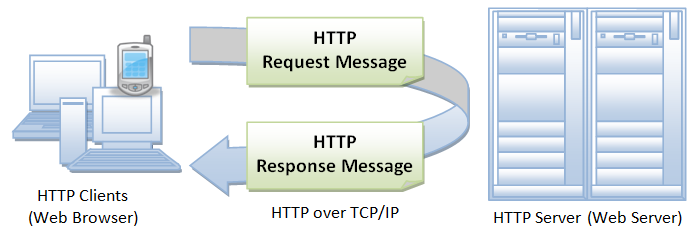
\includegraphics[scale=1.2]{slike/HTTP.PNG} %veličina slike u odnosu na originalnu datoteku i pozicija slike
    	\centering
    	\caption{Prikaz HTTP komunikacije između klijenta i poslužitelja}
    	\label{fig:promjene}
    \end{figure}
    
    \textit{\newline \newline}
    
    \textit{Naša grupa je za projekt na predmetu Programsko inženjerstvo (ak.god. 2023./2024.) odabrala React sustav za potrebe frontenda. Odabrali smo React zbog njegove jednostavne i moćne arhitekture koja omogućuje brz i održiv razvoj web aplikacija. React se temelji na principu komponenata, što znači da aplikaciju gradimo kao skup neovisnih dijelova sučelja, svaki s vlastitom logikom i stilovima. Time svaka komponenta postaje ponovno upotrebljiva i lako zamjenjiva što olakšava razvoj aplikacije.}
    
    \textit{Za backend smo odabrali raditi u programskom jeziku Java i to u Spring Boot-u. Koristili smo Maven alat za izgradnju programskog koda. Spring Boot nam se svidio zbog dvije karakteristike: inverzija kontrole gdje sam Spring Boot kontrolira izvršavanje programskog koda te injektiranje objekata o kojima ovisi rad koda. Neke od karakteristika Spring Boot-a su: unaprijed pripremljene funkcionalnosti, nema generiranja klasa i koda već se koriste unaprijed definirane biblioteke. U svakom slučaju Spring Boot zna dosta olakšati programeru posao. Također olakšava i spajanje na bazu podataka o kojoj će biti više riječi u sljedećoj cjelini.}
    
    \textit{Razvojno okruženje koje smo koristili zavisilo je od člana do člana ekipe, neki su radili u Eclipse-u, neki u IntelliJ. Koristili smo GitHub sustav za upravljanje verzijama programske potpore te TeXstudio za pisanje dokumentacije.}
    
    \begin{figure}[H]
    	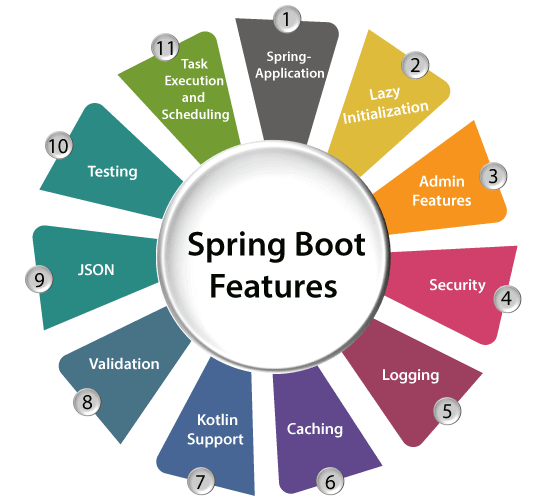
\includegraphics[scale=0.5]{slike/SpringBoot.PNG} %veličina slike u odnosu na originalnu datoteku i pozicija slike
    	\centering
    	\caption{Neke od koristi Spring Boot-a}
    	\label{fig:promjene}
    \end{figure}
		

				
		\section{Baza podataka}
			
			\textbf{\textit{dio 1. revizije}}\\
			
		\textit{Potrebno je opisati koju vrstu i implementaciju baze podataka ste odabrali, glavne komponente od kojih se sastoji i slično.}
		
			\subsection{Opis tablica}
			

				\textit{Svaku tablicu je potrebno opisati po zadanom predlošku. Lijevo se nalazi točno ime varijable u bazi podataka, u sredini se nalazi tip podataka, a desno se nalazi opis varijable. Svjetlozelenom bojom označite primarni ključ. Svjetlo plavom označite strani ključ}
				
				
				\begin{longtblr}[
					label=none,
					entry=none
					]{
						width = \textwidth,
						colspec={|X[6,l]|X[6, l]|X[20, l]|}, 
						rowhead = 1,
					} %definicija širine tablice, širine stupaca, poravnanje i broja redaka naslova tablice
					\hline \SetCell[c=3]{c}{\textbf{korisnik - ime tablice}}	 \\ \hline[3pt]
					\SetCell{LightGreen}IDKorisnik & INT	&  	Lorem ipsum dolor sit amet, consectetur adipiscing elit, sed do eiusmod  	\\ \hline
					korisnickoIme	& VARCHAR &   	\\ \hline 
					email & VARCHAR &   \\ \hline 
					ime & VARCHAR	&  		\\ \hline 
					\SetCell{LightBlue} primjer	& VARCHAR &   	\\ \hline 
				\end{longtblr}
				
				
			
			\subsection{Dijagram baze podataka}
				\textit{ U ovom potpoglavlju potrebno je umetnuti dijagram baze podataka. Primarni i strani ključevi moraju biti označeni, a tablice povezane. Bazu podataka je potrebno normalizirati. Podsjetite se kolegija "Baze podataka".}
			
			\eject
			
			
		\section{Dijagram razreda}
		
			\textit{Potrebno je priložiti dijagram razreda s pripadajućim opisom. Zbog preglednosti je moguće dijagram razlomiti na više njih, ali moraju biti grupirani prema sličnim razinama apstrakcije i srodnim funkcionalnostima.}\\
			
			\textbf{\textit{dio 1. revizije}}\\
			
			\textit{Prilikom prve predaje projekta, potrebno je priložiti potpuno razrađen dijagram razreda vezan uz \textbf{generičku funkcionalnost} sustava. Ostale funkcionalnosti trebaju biti idejno razrađene u dijagramu sa sljedećim komponentama: nazivi razreda, nazivi metoda i vrste pristupa metodama (npr. javni, zaštićeni), nazivi atributa razreda, veze i odnosi između razreda.}\\
			
			\textbf{\textit{dio 2. revizije}}\\			
			
			\textit{Prilikom druge predaje projekta dijagram razreda i opisi moraju odgovarati stvarnom stanju implementacije}
			
			
			
			\eject
		
		\section{Dijagram stanja}
			
			
			\textbf{\textit{dio 2. revizije}}\\
			
			\textit{Potrebno je priložiti dijagram stanja i opisati ga. Dovoljan je jedan dijagram stanja koji prikazuje \textbf{značajan dio funkcionalnosti} sustava. Na primjer, stanja korisničkog sučelja i tijek korištenja neke ključne funkcionalnosti jesu značajan dio sustava, a registracija i prijava nisu. }
			
			
			\eject 
		
		\section{Dijagram aktivnosti}
			
			\textbf{\textit{dio 2. revizije}}\\
			
			 \textit{Potrebno je priložiti dijagram aktivnosti s pripadajućim opisom. Dijagram aktivnosti treba prikazivati značajan dio sustava.}
			
			\eject
		\section{Dijagram komponenti}
		
			\textbf{\textit{dio 2. revizije}}\\
		
			 \textit{Potrebno je priložiti dijagram komponenti s pripadajućim opisom. Dijagram komponenti treba prikazivati strukturu cijele aplikacije.}